I test di integrazione servono ad assicurare che le varie componenti funzionino correttamente quando messe in relazione.


\subsubsection{Test di integrazione previsti}

\begin{tabularx}{\textwidth}{cXc}
	
	\rowcolor{greySWEight}
	
	\rowcolor{greySWEight}
	\textcolor{white}{\textbf{Codice}} & 
	\textcolor{white}{\textbf{Descrizione}} &
	\textcolor{white}{\textbf{Stato}} \\

\textbf{TI001} & Verifica il corretto funzionamento tra UsersRepository e MongoDB & \textcolor{ForestGreen}{Superato} \\
\textbf{TI002} & Verifica il corretto funzionamento tra PhraseRepository e MongoDB & \textcolor{ForestGreen}{Superato} \\
\textbf{TI003} & Verifica il corretto funzionamento tra ExerciseRepository e MongoDB & \textcolor{ForestGreen}{Superato} \\
\textbf{TI004} & Verifica il corretto funzionamento tra UserService e UsersRepository & \textcolor{ForestGreen}{Superato} \\
\textbf{TI005} & Verifica il corretto funzionamento tra PhraseService e PhraseRepository & \textcolor{ForestGreen}{Superato} \\
\textbf{TI006} & Verifica il corretto funzionamento tra ExerciseService e ExerciseRepository & \textcolor{ForestGreen}{Superato} \\
\textbf{TI007} & Verifica il corretto funzionamento tra SolutionService e la connessione a FreeLing & \textcolor{ForestGreen}{Superato} \\
\textbf{TI008} & Verifica il corretto funzionamento tra Controller e UserService & \textcolor{ForestGreen}{Superato} \\
\textbf{TI009} & Verifica il corretto funzionamento tra Controller e SolutionService & \textcolor{ForestGreen}{Superato} \\
\textbf{TI010} & Verifica il corretto funzionamento tra Controller e ExerciseService & \textcolor{ForestGreen}{Superato} \\
\textbf{TI011} & Verifica il corretto funzionamento tra AdminDevDashBoard e lo store	& Non Implementato	\\
\textbf{TI012} & Verifica il corretto funzionamento tra AdminUserDashBoard e lo store	& Non Implementato	\\
\textbf{TI013} & Verifica il corretto funzionamento tra Dashboard e lo store	 & \textcolor{ForestGreen}{Superato} \\
\textbf{TI014} & Verifica il corretto funzionamento tra DeveloperDashBoard e lo store	 & \textcolor{ForestGreen}{Superato} \\	
\textbf{TI015} & Verifica il corretto funzionamento tra DoneHomework e lo store	 & \textcolor{ForestGreen}{Superato} \\
\textbf{TI016} & Verifica il corretto funzionamento tra Homework e lo store	 & \textcolor{ForestGreen}{Superato} \\
\textbf{TI017} & Verifica il corretto funzionamento tra HomeworkExecution e lo store	 & \textcolor{ForestGreen}{Superato} \\
\textbf{TI018} & Verifica il corretto funzionamento tra InsertExercise e lo store	 & \textcolor{ForestGreen}{Superato} \\
\textbf{TI019} & Verifica il corretto funzionamento tra NewExercise e lo store	 & \textcolor{ForestGreen}{Superato} \\
\textbf{TI020} & Verifica il corretto funzionamento tra PublicExercise e lo store	 & \textcolor{ForestGreen}{Superato} \\
\textbf{TI021} & Verifica il corretto funzionamento tra Navbar e lo store	 & \textcolor{ForestGreen}{Superato} \\
				

	\rowcolor{white}
	\caption{Test di integrazione}
	\label{tab:tabellatestintegrazione}
\end{tabularx}

% \begin{figure}[H]
% 	\centering
% 	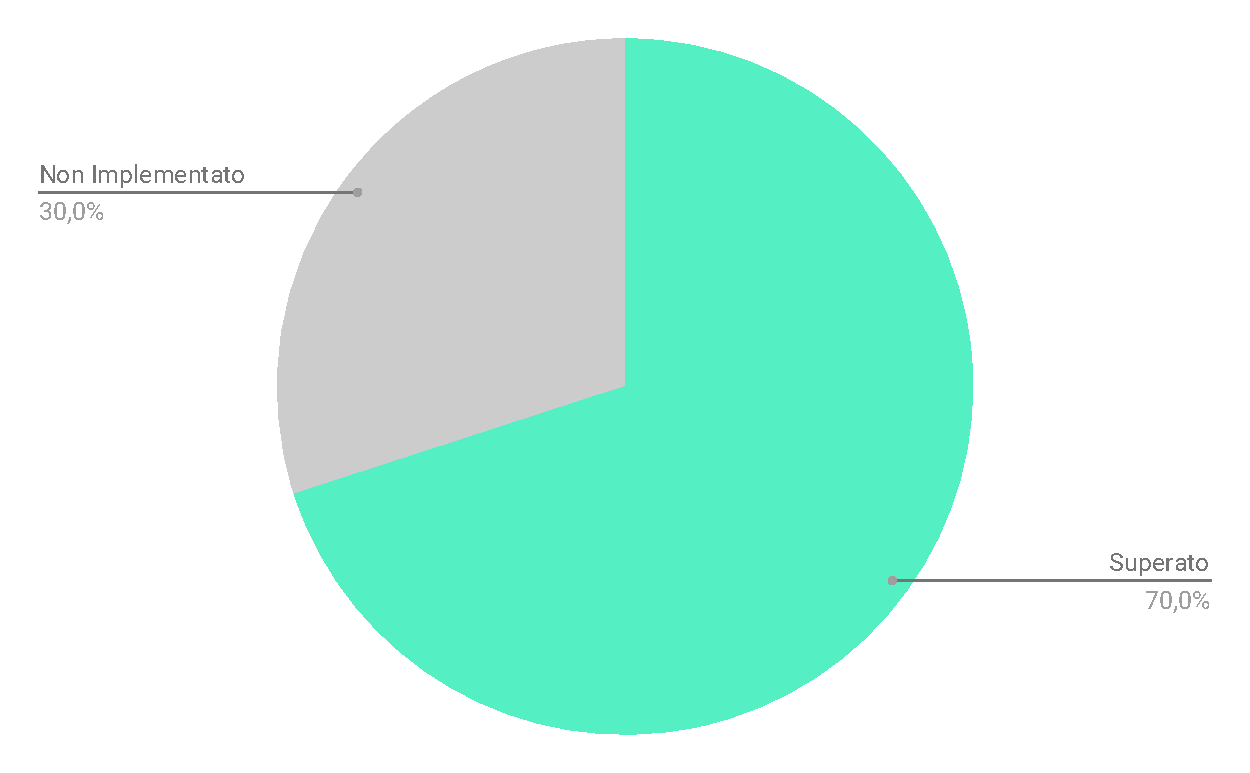
\includegraphics[width=0.7\linewidth]{sez/test/img/statoTestIntegrazione.pdf}
% 	\caption{Riepilogo stato test di integrazione}
% \end{figure}

\subsubsection{Tracciamento Test di integrazione - Componenti}

\begin{tabularx}{\textwidth}{cX}
	
	\rowcolor{greySWEight}
	
	\rowcolor{greySWEight}
	\textcolor{white}{\textbf{Test}} & 
	\textcolor{white}{\textbf{Componenti}} \\
	
	TI001 & colletta::repository::user::UsersRepository \\
	TI002 & colletta::repository::phrase::PhraseRepository \\
	TI003 & colletta::repository::exercise::ExerciseRepository \\
	TI004 & colletta::service::user::UserService \\
	TI005 & colletta::service::PhraseService \\
	TI006 & colletta::service::ExerciseService \\
	TI007 & colletta::service::SolutionService \\
	TI008 & colletta::controller::Controller \\
	TI009 & colletta::controller::Controller \\
	TI010 & colletta::controller::Controller \\
	TI011 & src::view::containers::DashboardContainers::AdminDevDashboard \\
	TI012 & src::view::containers::DashboardContainers::AdminUserDashboard \\
	TI013 & src::view::containers::DashboardContainers::Dashboard \\
	TI014 & src::view::containers::DashboardContainers::DeveloperDashboard \\
	TI015 & src::view::containers::ExerciseContainer::DoneHomework \\
	TI016 & src::view::containers::ExerciseContainer::Homework \\
	TI017 & src::view::containers::ExerciseContainer::HomeworkExecution \\
	TI018 & src::view::containers::ExerciseContainer::InsertExercise \\
	TI019 & src::view::containers::ExerciseContainer::NewExercise \\
	TI020 & src::view::containers::ExerciseContainer::PublicExercise \\
	TI021 & src::view::containers::NavbarContainers::Navbar \\

	\rowcolor{white}
	\caption{Tracciamento test di integrazione - componenti}
	\label{tab:tracciamentotestintegrazione}
\end{tabularx}
